\documentclass{beamer}

\usetheme{Warsaw}
%\usepackage[spanish]{babel}
\usepackage[latin1]{inputenc}
\usepackage{algorithm}
\usepackage{algorithmic}
\usepackage{verbatim}
\usepackage{amsbsy}
\usepackage{amsfonts}
\usepackage{amssymb}
\usepackage{multirow}
%\usepackage[dvipdf]{graphicx}

\setbeamercovered{transparent}

\newcommand{\?}{?`}
\newtheorem{definicion}{Definici\'on}

\mode<presentation>
{
  \setbeamertemplate{background canvas}[vertical shading][bottom=white!10,top=blue!10]
  \setbeamercolor{itemize item}{fg=red}
  \usetheme{CambridgeUS}
  \usefonttheme[onlysmall]{structurebold}
}

%
% The following info should normally be given in you main file:
%

\title[VAR-PLS]{VAR-PLS}
\author[Graciela Gonz\'alez Far\'ias] {Graciela Gonz\'alez Far\' ias}
\institute[CIMAT Monterrey]{CIMAT Monterrey\\
Monterrey, NL.}
\date{Mayo 2012}


\begin{document}


%\frame{\titlepage}

%%%%%%%%%%%%%%%%%%%%%%%%%%%%%%%%%%%%%%%%%%

\begin{frame}
  \begin{center}
    % \vspace{8mm}
    \begin{block}{}
      \begin{center}
        \vspace{3mm}
        {\Large Var PLS}
        \vspace{3mm}
      \end{center}
    \end{block}
    \vspace{5mm}
    Graciela Gonz\'alez Far\'ias \\
    \vspace{5mm}
    {\small Francisco Corona and Jes\'us Gonzalo \\
    Centro de Investigaci\'on en Matem\'aticas,
      Campus Monterrey\\
      ISBIS 2012\\
      Bangkok, Thailand, June 17, 2012}
    \vspace{5mm}
  \end{center}
\end{frame}


\begin{frame}{Contenido}
  \begin{itemize}
  \item Motivation
  \item PLSAR and PLS
  \item Quick overview of VAR Models
  \item Definition for VAR-PLS
  \item Bootstrap for VAR-PLS
  \item Conclusions
  \end{itemize}
\end{frame}

\begin{frame}{Motivaci\'on}
  \begin{itemize}
    \item PLS is a technique that has bee proven its impact on many applications such as quality control starting with the Chemistry, batch processes, medical images analysis, microarrays, path modeling, classification, discrimination, spacio-temporal PLS models just to mention some, with authors such as McGregor, Nomikos, MacIntosh, V. Esposito Vinz, P. Garthwaite, and so on 
    \item The method can be used in univariate and multivariate data as well
    \item {\it{It has been shown that gives better prediction even when the standard assumptions are met}}
    \item Phillip Hans Franses (2006) propose a methodology to construct the forecast $h$ steps ahead in an optimal way, through an autoregresive order $p$:  {\it{An Autoregresive Partial Least Square denote as  $PLSAR(h,p)$}}
      \end{itemize}
    \end{frame}

\begin{frame}{Our case of interest}
  \begin{itemize}
    \item Develop a model to predict the Mexican inflation, as precise as possible
    \item The model has to consider, as the principal source of the mexican inflation, the grow and the variation on the monetary condition of the country
    \item Irrespective of all possible discussions, there seems to be a common understanding to belived that the inflationary process, in the lung run, is a purely monetary fenomena
    \item Here we are not taking the discussion on the existence or not of such relationship but we will show its empirical properties with a model that is tested out of the sample via its error prediction measure
    
  \end{itemize}
\end{frame}

\begin{frame}{Our case of interest}
  We work with 4 indexes ( we bulit those) from January 2000 to Feb 2012
  \bigskip
  
  \begin{itemize}
    \item $p$: Consumer price index  
    \bigskip
    \item $m0$: Monetary base 
      \bigskip
    \item $r$: Equilibrium interest rate (28 days)
      \bigskip
    \item $y$: Industrial production index 
  \end{itemize}
\end{frame}

\begin{frame}{Nuestro caso de inter\'es}
  \begin{figure}[htbp]
    \center{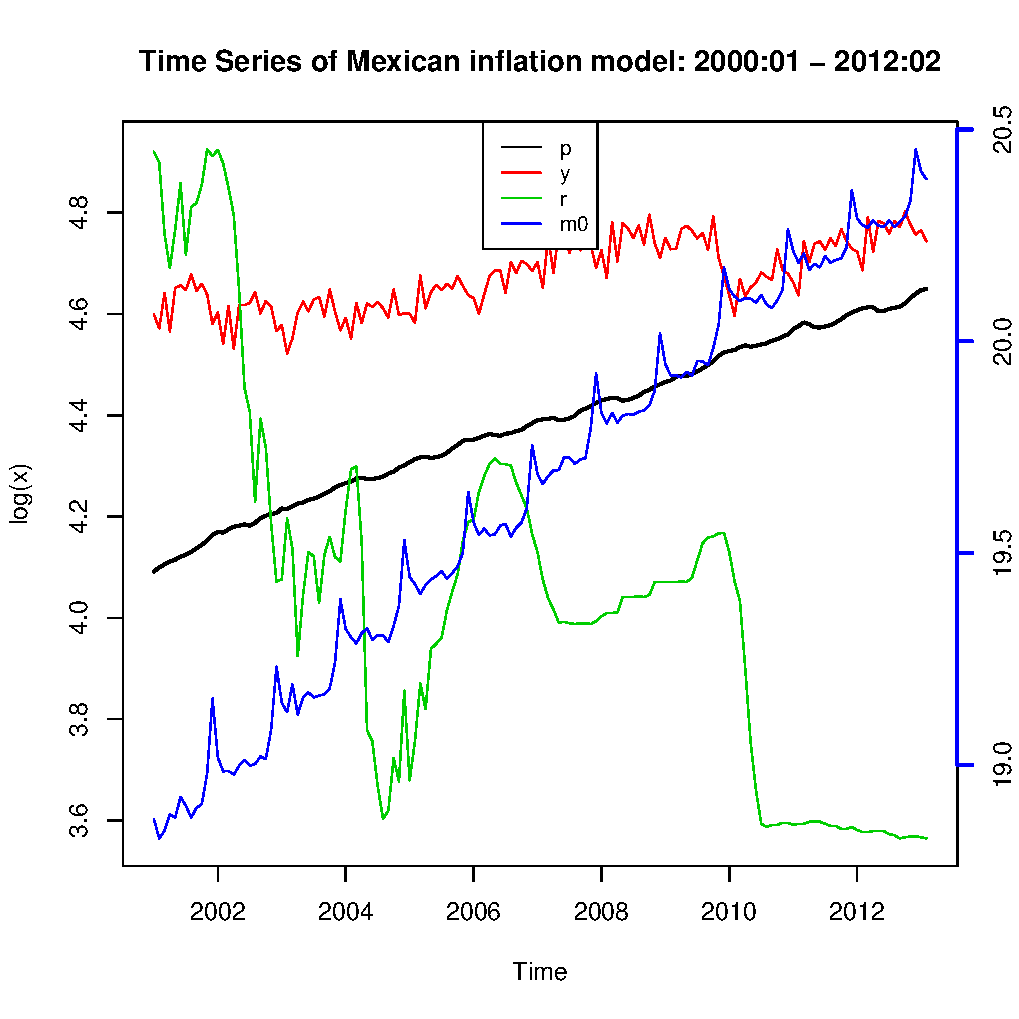
\includegraphics[scale=0.5]
      {figs/graph_1_v2.pdf}}
\end{figure}
\end{frame}

\begin{frame}{Our case of interest}
  \begin{itemize}
    \item We generalized the work proposed by Franses in the following way:
    \bigskip
    
      \begin{enumerate}
      \item Give a multivariate representation based on the flexibility of the $VAR$ models, model that we will call $VAR-PLS(h,p)$
      \item Extend the model to consider deterministic variables (dummies, trend, etc.) as well as exogenous variables
      \item Bootstrap prediction intervals
      \item Compare the forecast capabilities between a $VAR-PLS(h,p)$ and a forecast $VAR$ model explicitly built for (integral predictor method)
            \end{enumerate}
  \end{itemize}
\end{frame}

\begin{frame}{}
  \begin{block}{}
    \begin{center}
      \vspace{3mm}
      {\Large $PLSAR(h,p)$}
      \vspace{3mm}
    \end{center}
  \end{block}
\end{frame}

\begin{frame}{$PLSAR(h,p)$}
  Franses three different ways to construct a forecast for an $AR(p)$:
  \bigskip
  \begin{itemize}
    \item[\textbf{1-}] A single model for all horizons , an iterative procedure will come on hand
      \begin{displaymath}
        AR(p): y_{T+h}=\mu+
        \rho_1y_{T+h-1}+\rho_2y_{T+h-2}+\cdots + \rho_py_{T+h-p} + \epsilon_T
      \end{displaymath}
      
      For the $AR(p)$ the classical procedure to get $h$
      step ahead forecast, plus the fact that we estimate the parameters (OLS).
  \end{itemize}
\end{frame}

\begin{frame}{$PLSAR(h,p)$}
  \begin{itemize}
  \item[\textbf{2-}] One model for each horizon, the variance will vary within each horizon and {\it{one can count with different models for each step}}
  \bigskip
    \begin{displaymath}
      AR_h(p): y_{t+h}=\mu+
      \rho_{1,h}y_{t}+\rho_{2,h}y_{t-1}+\cdots + \rho_py_{t-p}+\epsilon_{t,h}
    \end{displaymath}
    The $AR_h(p)$  is an alternative to the $AR(p)$ because
    \begin{itemize}
    \item OLS minimize the sum of square of $\epsilon_t$  but there is no way to assure it will remain minimum for all the $h$ steps in the future 
    \item For stationary time series recall the the forecast of an  $AR(p)$ model quickly converge to the inconditional mean (and variance, for the interval prediction error) clearly depending on  
    $h\geq p$
        \item For more details on this type of models see : Pesaran \& Pick (2010), Marcellino, Stock \& Watson (2004), Carreiro, Kapetorios \& Marcellino (2010), Tiao \& Xu (1993) among others.
    \end{itemize}
  \end{itemize}
\end{frame}

\begin{frame}{$PLSAR(h,p)$}
  \begin{itemize}
  \item[\textbf{3-}] Something in between: $PLSAR$, this model behaves like {\it{ in the middle }}between an $AR(p)$ and a $AR_h(p)$  
    \begin{displaymath}
      PLSAR(h,p): \hat{Y}=XB_{PLS}
    \end{displaymath}
    \begin{itemize}
    \item It is clear that exists adjacent correlation between the time series, and neither one of the above models take them into account. In other words, we know that $(y_t,y_{t-j})$ are correlated and so are $(y_{T+h},y_{T+h-j})$, . Therefore we would like to jointly predict $(y_{t+h},y_{t+h-1},y_{t+h-2},\ldots,y_{t+1})$ through $(y_{t},y_{t-1},y_{t-2},\ldots,y_{t-p})$. PLS is a techinique very atractive to do so.
    \end{itemize}
  \end{itemize}
\end{frame}

\begin{frame}{$PLSAR(h,p)$}
  \begin{itemize}
  \item[\textbf{3-}]   Franses propose to arrange the information as 

      \begin{displaymath}
        (y_{t},y_{t-1},y_{t-2},\ldots,y_{t-p}) \text{ as the predictor matrix
           } X
      \end{displaymath}
      \begin{displaymath}
        (y_{t+h},y_{t+h-1},y_{t+h-2},\ldots,y_{t+1})
        \text{ as the predicted matrix } Y
      \end{displaymath}
      \bigskip
      \item Applied the $PLS$ algorithm, to get the latent variables with the relevant information given in $X $ and $Y$.
      \medskip
     \item His simulations shows that the $PLSAR(h,p)$ is quite competitive with respect to the classical models in the literature
  \end{itemize}
\end{frame}

\begin{frame}{}
  \begin{block}{}
    \begin{center}
      \vspace{3mm}
      {\Large $PLS$}
      \vspace{3mm}
    \end{center}
  \end{block}
\end{frame}

\begin{frame}{PLS}
  \begin{itemize}
  \item PLS can be tract from different stand points, to us the relationship between its linear expression  will be the best one, in order to related with a Vector Autoregresive model   
   \bigskip
  
   \begin{displaymath}
      Y=XB+U,
    \end{displaymath}
    \bigskip
    where $Y$ is a $N\times k$ matrix, $X$ is $N\times p$, $B$ is a
     $p\times k$ matrix, and  $U$ is  $N\times k$.


  \end{itemize}
\end{frame}


 
\begin{frame}{PLS}
  \begin{itemize}
  \item The basic procedure maximize the  
    \begin{displaymath}
      \max cov(X\alpha,Y\beta)^2
    \end{displaymath}
    under certain restrictions,
    \begin{displaymath}
      \alpha'(S_{xx}^{*}+\lambda_x)\alpha = 1 \quad \text{and } \quad
      \beta'(S_{yy}^{*}+\lambda_y)\beta = 1 
    \end{displaymath}
    donde $S_{xx}^{*}=(1-\lambda_x)S_{xx}$ and
    $S_{yy}^{*}=(1-\lambda_y)S_{yy}$.
    \begin{itemize}
    \item $(X\alpha,Y\beta)$ are linear combinations of the variables that  maximize the covariance or actually the squere covariance (the sign is not important just the direction)
    \item $S_{xx}$ and $S_{yy}$ the varince covariance matrices
      , $\beta'\beta=1$ y $a'S_{xx}a=1$.
    \end{itemize}
  \end{itemize}
\end{frame}
 
\begin{frame}{PLS}
  \begin{itemize}
  \item We maximze the the objective function:
    \begin{displaymath}
      \mathcal{L}=
      (\alpha'S_{xy}\beta)^2-\gamma(\alpha'(S_{xx}+\lambda_x)\alpha-1)
      - \mu(\beta'(S_{yy}+\lambda_y)\beta-1).
    \end{displaymath}
  \item After some algebra we get the {\textcolor{blue}{scores}} for  $X$ y
    $Y$, $t=Xw=Ew$ and $u=Yq=Fq$.
  \item  Normalizing the scores   $t=t/\sqrt{t't}$, and after simplifications and more algebra we get the \textcolor{red}{loadings} for  $X$ and $Y$: $p=E't$
   and $q=F't$.
  \end{itemize}
\end{frame}
 
\begin{frame}{PLS}
  \begin{itemize}
  \item Writing in matrix form $w,t,p$ y $q$ we get $R=W(P'W)^{-1}$ and
   finally
    \begin{displaymath}
      Y=XB+U, \text{ then} \hat{Y}=XB_{PLS},
    \end{displaymath}
    where $B_{PLS}=R\textcolor{blue}{(T'T)^{-1}T'Y}=RQ'$.
  \item     \bigskip

    For a nice introduction see P.H. Garthwaite
    (1994). An Interpretation of Partial Least Squares. JASA Vol 89,
    No 425, pp 122-127 and A. Hoskuldsson (1988). PLS Regression Methods. Journal of
    Chemometrics, Vol 2, pp 221-228.\\
    \medskip
    \textcolor{blue}{Note}: Franses shows that if  the $B_{PLS}$ matrix has full rank it implies a different model for
each of the columns of $Y$ , and hence a model like $AR_{h,p}$. In the exceptional case that
$B_{PLS}$ has rank 1, then the $AR(p)$ appears.
  \end{itemize}
\end{frame}

\begin{frame}{}
  \begin{block}{}
    \begin{center}
      \vspace{3mm}
      {\Large Vector Autoregressive models and PLS}
      \vspace{3mm}
    \end{center}
  \end{block}
\end{frame}

\begin{frame}{$VAR-PLS$}
  Un proceso $VAR(p)$ se define como
    \begin{displaymath}
      y_t=A_1y_{t-1} + A_2y_{t-2} + \cdots + A_py_{t-p} + CD_t + u_t,
    \end{displaymath}
    donde
    \begin{itemize}
    \item $A_i$, $i=1,2,\ldots, p$, son matrices de coeficientes
    \item $u_t$ es un proceso de ruido blanco con matriz de
      covarianzas $\Sigma_u=E(u_t,u_t')$
    \item $C$ es una matriz de regresores deterministicos
    \item $D_t$ es un vector de regresores determin\'isticos apropiados
    \end{itemize}
\end{frame}

\begin{frame}{$VAR-PLS$}
  Notemos que el $Var(p)$ puede definirse como un $Var(1)$ mediante 
    \begin{displaymath}
      Y_t=AY_{t-1} + V_t,
    \end{displaymath}
    con
    \begin{small}
    \begin{displaymath}
      Y_t=\left(
        \begin{array}{c}
          y_t \\
          y_{t-1} \\
          \vdots \\
          y_{t-p+1}
        \end{array}
        \right), \quad
        A=\left(
        \begin{array}{ccccc}
          A_1 & A_2 & \cdots & A_{p-1} & A_p \\
          I & 0 & \cdots & 0 & 0 \\
          0 & I & \cdots & 0 & 0 \\
          \vdots & \vdots & \ddots & \vdots & \vdots \\
          0 & 0 & \cdots & I & 0
        \end{array}
        \right), \quad
        V_t=\left(
        \begin{array}{c}
          u_t \\
          0 \\
          \vdots \\
          0
        \end{array}
        \right).
    \end{displaymath}
    \end{small}
    Si los valores propios de $A$ son menores que 1, entonces el
    proceso $Var(p)$ es estable.
\end{frame}

\begin{frame}{$VAR-PLS$}
  \begin{itemize}
  \item Un procedimiento para encontrar el orden $p$ del modelo
    consiste en ordenar los $p=0,\ldots,p_{\max}$ y elegir el valor
    $p$ que minimice cierto criterio de informaci\'on de la forma
    \begin{displaymath}
      IC(p)-\log \vert \hat{\Sigma(p)} \vert + C_T \varphi(K,p),
    \end{displaymath}
    donde
    \begin{itemize}
      \item $\hat{\Sigma(p)}=T^{-1} \sum_{i=1}^T\hat{u}_t'\hat{u}_t$,
      \item $C_T$ es una secuencia indexada por el n\'umero de
        realizaciones de $T$
      \item $\varphi(K,p)$ es una funci\'on que penaliza la
        complejidad del modelo
    \end{itemize}
  \end{itemize}
\end{frame}

\begin{frame}{$VAR-PLS$}
  \begin{itemize}
  \item Los cuatro criterios de informaci\'on m\'as utilizados son
    \begin{itemize}
    \item Akaike: $AIC(p)=\vert \hat{\Sigma(p)} \vert +
      \frac{2}{t}pK^2$
    \item Schwartz-Bayesiano: $BIC(p)=\vert \hat{\Sigma(p)} \vert +
      \frac{\log T}{t}pK^2$
    \item Hannan-Quinn: $HQ(p)=\vert \hat{\Sigma(p)} \vert +
      \frac{2\log T}{t}pK^2$
    \item Error final de predicci\'on:
      $FPE(p)=\left(\frac{T+p^{*}}{T-p^{*}}\right)^K
      \text{det}(\hat{\Sigma(p)})$  
    \end{itemize}
  \item El criterio AIC sobreestima asint\'oticamente el orden con
    probabilidad positiva, mientras que BIC y HQ estima
    consistentemente el orden cuando el verdadero valor de $p\leq
    p_{max}$. 
  \end{itemize}
\end{frame}

\begin{frame}{$VAR-PLS$}
  Notemos que al igual que el caso univariado, podemos pronosticar
  recurs\'ivamente mediante
  \begin{displaymath}
    y_{T+h\setminus T}=A_1y_{T+h-1} + \cdots + A_py_{T+h-p} + CD_{T+h}
  \end{displaymath}
  \begin{itemize}
  \item La estimaci\'on de $A_i$ se realiza generalmente mediante OLS
    \begin{displaymath}
        vec(\hat{A})=\left(
        \begin{array}{c}
          \hat{A}_1 \\
          \vdots \\
          \hat{A}_p
        \end{array}
        \right).      
    \end{displaymath}
  \end{itemize}
\end{frame}

\begin{frame}{$VAR-PLS$}
  \begin{itemize}
  \item Bajo ciertas condiciones de generalidad del comportamiento
    estacionario y ergodicidad en los modelos VAR (Hamilton, 1994,
    Lutkepohl, 1991), $vec(\hat{A})$ es consistente y distribuido
    asint\'oticamente con matriz de covarianzas
    \begin{displaymath}
      \widehat{var}\left(vec(\hat{A})\right)=\hat{\Sigma} \otimes
      (Z'Z)^{-1},
    \end{displaymath}
    donde
    \begin{displaymath}
      \hat{\Sigma}=\frac{\sum_{t=1}^T\hat{\epsilon}_t'\hat{\epsilon}_t}{T-K}
    \end{displaymath}
    y
    \begin{displaymath}
      \hat{\epsilon}_t=Y_t-\hat{A}'Z_t=Y_t-\hat{A}'Y_t
    \end{displaymath}
    es el residual de m\'inimos cuadrados al tiempo $t$.
  \end{itemize}
\end{frame}

\begin{frame}{$VAR-PLS$}
  \begin{itemize}
  \item El $i-$\'esimo elemento de $vec(\hat{A})$ es asint\'oticamente
    normal (para un $VAR$ estable) con errores est\'andar dados por la
    ra\'iz cuadrada de los elementos de la diagonal de $\hat{\Sigma}
    \otimes (Z'Z)^{-1}$.
    \item Las pruebas $t$ son v\'alidas asint\'oticamente para los
      coeficientes estimados.
  \end{itemize}
\end{frame}

\begin{frame}{$VAR-PLS$}
  Una situaci\'on de inter\'es sucede cuando existen una o m\'as
  ra\'ices unitarias en las $y_j'$s. Esto ha originado una teor\'ia
  econ\'omica que se basa en modelar el comportamiento de largo plazo
  y analizar la din\'amica temporal de un conjunto de series.
  \begin{itemize}
  \item \textbf{Cointegraci\'on: } Las componentes del vector $y_t$ se
    dice que son cointegradas de orden $d,b$, lo cual denotamos con
    $y_t\sim CI(d,b)$, si
    \begin{enumerate}
    \item todos los componentes de $y_t\sim$ son $I(d)$
    \item existe un vector $\beta\neq 0$ tal que $z_t=\beta'y_t\sim
      I(d-b)$, $b>0$. El vector $\beta$ es llamado vector de
      cointegraci\'on. 
    \end{enumerate}
  \end{itemize}
\end{frame}

\begin{frame}{$VAR-PLS$}
  \begin{itemize}
  \item \textbf{Correcci\'on de error: } Consideremos el vector bivariado
    $y_t=(y_{1t},y_{2t})'$ con vector de cointegraci\'on
    $\beta=(1-\beta_2)'$, entonces $\beta'y_t=y_{1t}-\beta_2y_{2t}\sim
    I(0)$ y existe una representaci\'on de correcci\'on de error de
    \begin{enumerate}
    \item $\Delta y_{1t}=\alpha_1+\gamma_1(y_{1t-1}-\beta_2y_{2t-1})+
      \sum_{i=1}^K \psi_{1,i}\Delta y_{1t-i} + \sum_{i=1}^K
      \psi_{2,i}\Delta y_{2t-i} + u_{1t}$ 
    \item $\Delta y_{2t}=\alpha_2+\gamma_2(y_{1t-1}-\beta_2y_{2t-1})+
      \sum_{i=1}^L \xi_{1,i}\Delta y_{1t-i} + \sum_{i=1}^L
      \xi_{2,i}\Delta y_{2t-i} + u_{2t}$ 
    \end{enumerate}
  \end{itemize}
  
\end{frame}

\begin{frame}{$VAR-PLS$}
  Notemos que el modelo $VAR(p)$ puede expresarse como
  \begin{displaymath}
    \Delta y_{t}=\Pi y_{t-1}+\Gamma_1 \Delta y_{t-1} + \cdots +
    \Gamma_{p-1} \Delta y_{t-p+1} + CD_t + u_t,
  \end{displaymath}
  donde $\Gamma_i=-(A_{i+1}+\cdots + A_p)$, para $i=1,\ldots ,p-1$ y
  $\Pi=-(I-A_1-A_2-\cdots - A_p)$. 

  Lo anterior es llamado Modelo de
  Vector de Correcci\'on de Error (VECM) transitorio.

  O bien como
  \begin{displaymath}
    \Delta y_t=\Pi y_{t-p}+\Gamma_1 \Delta y_{t-1} + \cdots +
    \Gamma_{p-1} \Delta y_{t-p+1} + CD_t + u_t,
  \end{displaymath}
  donde $\Gamma_i=-(I-A_{1}-A_2-\cdots -A_i)$, para $i=1,\ldots ,p-1$
  y $\Pi=-(I-A_1-A_2-\cdots - A_p)$. Este modelo es llamado VECM de
  largo plazo.

\end{frame}

\begin{frame}{$VAR-PLS$}
  La matriz $\Pi$ tiene las siguientes caracter\'isticas:
  \begin{enumerate}
  \item $rk(\Pi)=n$, todas las $n$ combinaciones deben ser
    estacionarias; el VECM es un modelo VAR en niveles
  \item $rk(\Pi)=0$, no existe una combinaci\'on lineal estacionaria
    tal que $\Pi y_{t-1}$ sea estacionaria, excepto la soluci\'on
    trivial, i.e, es un modelo $VAR(p-1)$ en primeras diferencias.
  \item $0<rk(\Pi)<n$, en este caso $\Pi=\alpha \beta'$ con
    dimensi\'on $n\times r$ y $\beta' y_{t-1}$ es estacionaria. Cada
    columna de $\beta$ representa una relaci\'on de largo plazo.
  \end{enumerate}

  \textbf{Si el objetivo es pronosticar, a\'un en el caso de variables
  integradas y cointegradas, hacerlo mediante la representaci\'on VAR
  es muy apropiado} (ver Lutkepohl, 2006).
\end{frame}

\begin{frame}{$VAR-PLS$}
  Del ejemplo, notamos que (VER ESTA PARTE!1!1)
  \begin{itemize}
  \item Se especific\'o el orden $p$ del $VAR$ te\'orica a trav\'es
    del criterio de Error Final de Predicci\'on, el cual fue de
    12. Tambi\'en se realiz\'o la prueba de Johansen para verificar la
    presencia de relaciones de largo plazo.
  \item Los resultados obtenidos mostraron que al 1\%, 5\% y 10\%
    existe una ecuaci\'on de cointegraci\'on, la cual est\'a dada por
    la siguiente expresi\'on:
    \begin{displaymath}
      p+9.68-0.43m-0.89y+0.1r=0
    \end{displaymath}
  \item Lo anterior es congruente con la realidad, ya que establece
    que el traspaso inflacionario est\'a impulsado por el crecimiento
    monetario, exceso de demanda y la reducci\'on del costo del
    dinero. 
  \end{itemize}
\end{frame}

\begin{frame}{}
  \begin{block}{}
    \begin{center}
      \vspace{3mm}
      {\Large VAR-PLS}
      \vspace{3mm}
    \end{center}
  \end{block}
\end{frame}

\begin{frame}{$VAR-PLS$}
  \begin{itemize}
  \item Se propone utilizar la representaci\'on de un modelo VAR para
    el proceso generador de datos
  \item El modelo VAR determinar\'a el orden del proceso
    autorregresivo que ser\'a utilizado en la regresi\'on PLS
  \item Utilizaremos matrices en estructura de rezagos seg\'un cada
    una de las variables
  \end{itemize}
\end{frame}

\begin{frame}{$VAR-PLS$}
  \begin{itemize}
  \item Agrupamos en la matriz $X$ la informaci\'on observada en el
    pasado:
    \begin{displaymath}
      X=Y_{t-1}=\left(
        \begin{array}{c}
          y_{t-1} \\
          y_{t-2} \\
          \vdots \\
          y_{t-p}
        \end{array}
      \right), 
    \end{displaymath}
  \item En $Y$ lo observado en el tiempo $t$:
    \begin{displaymath}
      Y=Y_{t}=\left(
        \begin{array}{c}
          y_t \\
          y_{t-1} \\
          \vdots \\
          y_{t-p+1}
        \end{array}
      \right), 
    \end{displaymath}
    estimando el modelo mediante el proceso de construcci\'on de
    variables latentes.
  \end{itemize}
\end{frame}

\begin{frame}{$VAR-PLS$}
  \begin{itemize}
  \item Es f\'acil introducir variables ex\'ogenas o determin\'isticas
    mediante una matriz $C$, modificando la composici\'on de 
    \begin{footnotesize}
    \begin{displaymath}
      X=Y_{t-1}^{*}=\left(
        \begin{array}{c}
          y_{t-1} \\
          y_{t-2} \\
          \vdots \\
          y_{t-p} \\
          D_t
        \end{array}
      \right), 
    \end{displaymath}
    y por ende, de la matriz de coeficientes
    \begin{displaymath}
      A^{*}=\left(
        \begin{array}{cccccc}
          A_1 & A_2 & \cdots & A_{p-1} & A_p & C \\
          I & 0 & \cdots & 0 & 0 & 0 \\
          0 & I & \cdots & 0 & 0 & 0 \\
          \vdots & \vdots & \ddots & \vdots & \vdots \\
          0 & 0 & \cdots & I & 0 & 0
        \end{array}
        \right)
    \end{displaymath}
    \end{footnotesize}
  \item De esta forma obtenemos un modelo $VAR-PLSX$ con la \'unica
    finalidad de pronosticar $h$ pasos adelante.
  \end{itemize}
\end{frame}

\begin{frame}{$VAR-PLS$}
  Para el $VAR(p=3)-PLS(h=24,j)$
  \begin{itemize}
  \item Conservamos las 24 observaciones para tener un horizonte largo
    de posibles comparaciones.
  \item Consideramos variables dummies para los efectos mensuales.
  \item Para el \'optimo $p$ estimamos $VAR-PLS$. Usamos R para
    ajustar $Y_t(119\times 4)(119\times 23)B(23\times 4)+U(23\times
    4)$, y predecimos para el $VAR(3)-PLS(24,j)$ de forma recursiva
    como en el $VAR(p)$. Seg\'un el ejercicio de Franses, el \'ultimo
    componente concuerda con la estimaci\'on del $VAR(p)$ usando OLS.
  \item Para las $pK+g=23$ componentes y los 24 pasos fuera
    de muestra, obtuvimos el MAPE para realizar la comparaci\'on.
  \end{itemize}
\end{frame}

\begin{frame}{$VAR-PLS$}
  Para el modelo $VAR(p=3)$
  \begin{itemize}
  \item Combinamos las estimaciones de todas las variables en el
    $VAR_j(p)$, $j=1,2,\ldots,3696$
  \item Para los 24 pasos fuera de muestra usamos 7 criterios
    diferentes para medir el comportamiento del pron\'ostico (Hyndman
    \& Koehler, 2006):
    \begin{itemize}
    \item MAPE: Mean Absolute Percentage Error
    \item MdAPE: Median Absolute Percentage Error
    \item RMSPE: Root Mean Square Percentage Error
    \item RMdSPE: Root Median Square Percentage Error
    \item MRAE: Mean Relative Absolute Error
    \item MdRAE: Median Relative Absolute Error
    \item GMRAE: Geometric Mean Absolute Error
    \end{itemize}
  \end{itemize}
\end{frame}

\begin{frame}{$VAR-PLS$}
  \begin{itemize}
  \item Para los \'ultimos 3 criterios, necesitamos trabajar con un
    modelo benchmark (AR de orden 1) para $i=1,\ldots,24$,
    obteniendo el siguiente estad\'istico:
    \begin{displaymath}
      test=\frac{Y_{t-i}-Y_{t+i,VAR_j(p)}^f}{Y_{t+i}-Y_{t+i,AR(1)}^f}
    \end{displaymath}
  \item Para el \'ultimo criterio, integramos a uno tomando el cuantil
    0.5 para el horizonte considerado, y lo repetimos para sus
    intervalos de confianza superior e inferior.
  \end{itemize}
\end{frame}

\begin{frame}{}
  \begin{block}{}
    \begin{center}
      \vspace{3mm}
      {\Large Intervalo de predicci\'on: VAR-PLS}
      \vspace{3mm}
    \end{center}
  \end{block}
\end{frame}

\begin{frame}{$VAR-PLS$}
  Uno de los objetivos de este trabajo es la construcci\'on del
  intervalo de predicci\'on para el modelo VAR-PLS.

  El procedimiento es similar a lo propuesto por Pascual y
  colaboradores (2011), que a su vez, se basan en el
  trabajo de Kim (2001) y de Pascual y colaboradores (2004)

  Para el modelo VAR, ellos propusieron un m\'etodo que incluye:
  \begin{enumerate}
  \item La incertidumbre dada por la estimaci\'on del par\'ametro,
    donde se construyen regiones de confianza usando un m\'etodo Bootstrap
    \begin{enumerate}
    \item Estas regiones son v\'alidas bajo supuestos de Gaussianidad
      (L\"ukepolh et al, 1991), aunque no reflejen, para muestras
      peque\~nas, la distribuci\'on asint\'otica de los valores
      predichos (con los par\'ametros estimados)
    \end{enumerate}
  \item La representaci\'on hacia atr\'as complica mucho m\'as los
    c\'alculos en el caso de la representaci\'on $VAR(p)$, con $p$
    tomando valores mayores a 5, que es algo muy com\'un.
    \begin{enumerate}
    \item Pascual et al, muestra que la representaci\'on hacia atr\'as
      puede evitarse sin perder las buenas propiedades del
      procedimiento Bootstrap.
    \end{enumerate}
  \end{enumerate}
\end{frame}

\begin{frame}{$VAR-PLS$}
  Por supuesto, en nuestro caso, necesitamos adecuar el procedimiento
  para la representaci\'on VAR-PLS, lo cual se muestra a continuaci\'on:
  \begin{footnotesize}
  \begin{enumerate}
  \item Ajustar el modelo para estimar $Y_t=X_t\hat{B}_{PLS}$.
  \item Obtener los residuales estandarizados  $\hat{U}_t^{*}$ y la
    distribuci\'on emp\'irica de estos residuales.
  \item Con los $p$ valores iniciales $Y_0=\lbrace Y_p,\ldots,Y_1\rbrace$ y
    los valores obtenidos en los pasos 1 y 2, generar $Y_t^{*}$, que
    son los valores bootstrap, donde las $\hat{U}_t^{*}$ son muestras
    independientes generadas mediante su distribuci\'on emp\'irica:
    \begin{displaymath}
      Y_t^{*}=X_t\hat{B}_{PLS}+\hat{U}_t^{*}, \quad t=1,\ldots,n-p
    \end{displaymath}
  \item Continuamos de esta forma para obtener $\hat{Y}_{T+h}^{*}$,
    replicando los pasos 2 a 4, para $n=1,\ldots,N$.
  \item Para cada una de las $n$ variables y el conjunto de $N$
    pron\'osticos obtenemos
    \begin{displaymath}
      CI_{T+h}=\lbrace y_{n,T+k}|y_{n,T+k} \in
      [q_B^{*}(\tau),q_B^{*}(\tau-1)] \rbrace,
    \end{displaymath}
    donde $q_B^{*}(\tau)$ es el $\tau-$\'esimo percentil de
    $G_{n,B}^{*}(x)=\#\left(y_{n,T+k}^{*(b)}\leq x\right)/N$
  \end{enumerate}
  \end{footnotesize}
\end{frame}

\begin{frame}{$VAR-PLS$}
  \begin{figure}[htbp]
    \center{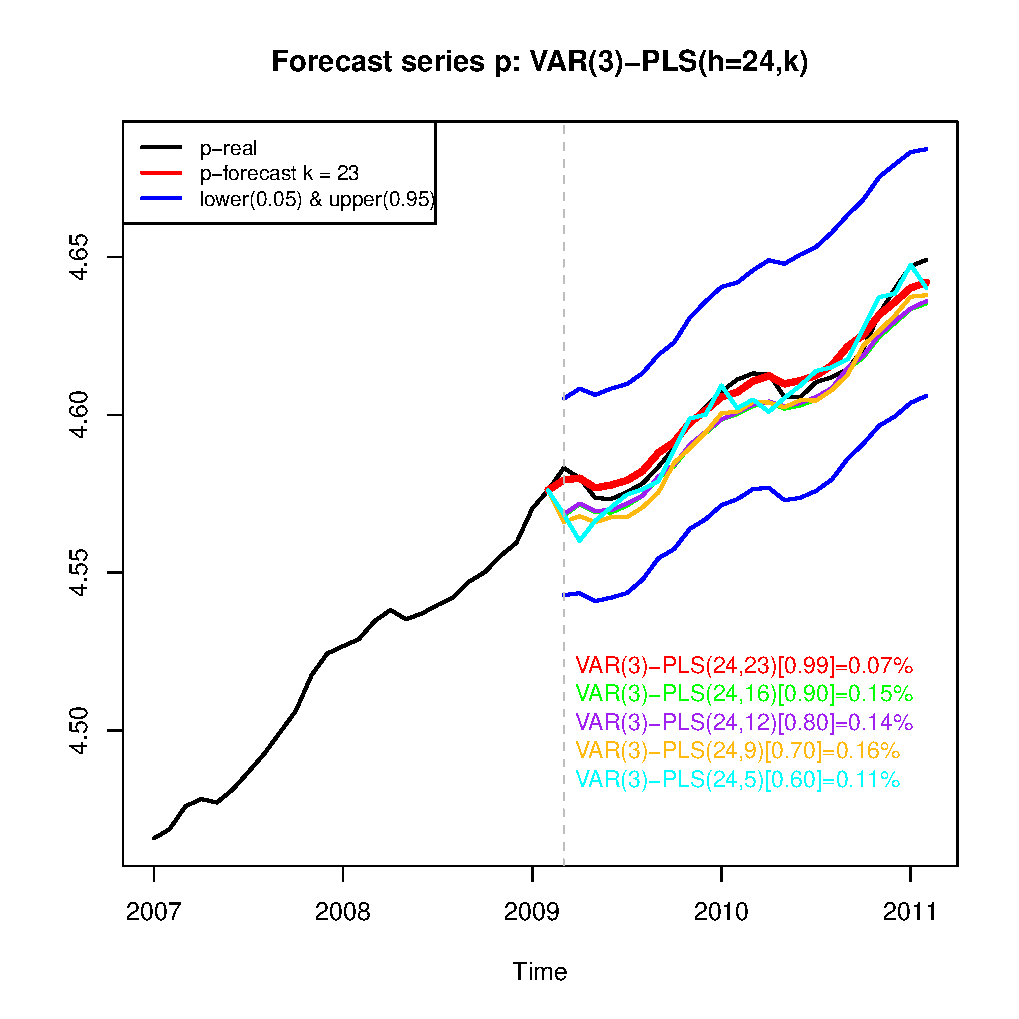
\includegraphics[scale=0.3]
      {figs/graph_2_v2.pdf}}
  \end{figure}
  \begin{footnotesize}
    \begin{itemize}
    \item Desde un punto de vista econ\'omico, esta aproximaci\'on es
      excelente. 
    \item Observamos que, ya sea que usemos $k=23$ (0.99 de la
      variabilidad) con un porcentaje de error de 0.07\%, o con 70\%
      de explicaci\'on con un porcentaje de error de 0.16\%, el valor
      real y el predicho, para efectos pr\'acticos, son casi
      id\'enticos.
    \item El intervalo Bootstrap tiene un muy buen comportamiento
    \end{itemize}
  \end{footnotesize}
\end{frame}

\begin{frame}{$VAR-PLS$}
  \textbf{Nota: }El objetivo es pronosticar el precio, sin embargo, ya
  que es un modelo multivariado, obtenemos tambi\'en el pron\'ostico
  para las otras 3 variables con error de predicci\'on (MAPE promedio)
  de \textbf{0.20\% para la base monetaria, 0.60\% para el \'indice de
    producci\'on industrial y 12.03\% para la tasa de equilibirio de
    inter\'es.}
\end{frame}

\begin{frame}{$VAR-PLS$}
  Para el Integral-VAR, los $VAR_J(P)$ \'optimos fueron los
  siguientes:
  \medskip

  \begin{footnotesize}
  \begin{tabular}{|l|c|c|c|c|}
    \hline
    Criterio & MAPE & MdAPE & RMSPE & RMdSPE \\
    \hline
    Estad\'istico & 0.16 & 0.12 & 0.19 & 0.12 \\
    Variable & r & r & r & r \\
    Lags & 3 & 2 & 3 & 2 \\
    Estacionalidad & 9 & 11 & 9 & 11 \\
    Especificaci\'on & ninguna & ninguna & ninguna& ninguna \\
    \hline
  \end{tabular}
  \end{footnotesize}

  \begin{footnotesize}
  \begin{tabular}{|l|c|c|c|}
    \hline
    Criterio & MRAE & MdRAE & GMRAE \\
    \hline
    Estad\'istico & 0.16 & 0.12 & 0.11 \\
    Variable & r & r & r \\
    Lags & 2 & 3 & 5 \\
    Estacionalidad & 6 & 9 & 11 \\
    & ninguna& ninguna& ninguna \\
    \hline
  \end{tabular}
  \end{footnotesize}
  \medskip
\end{frame}

\begin{frame}{$VAR-PLS$}
  \begin{figure}[htbp]
    \center{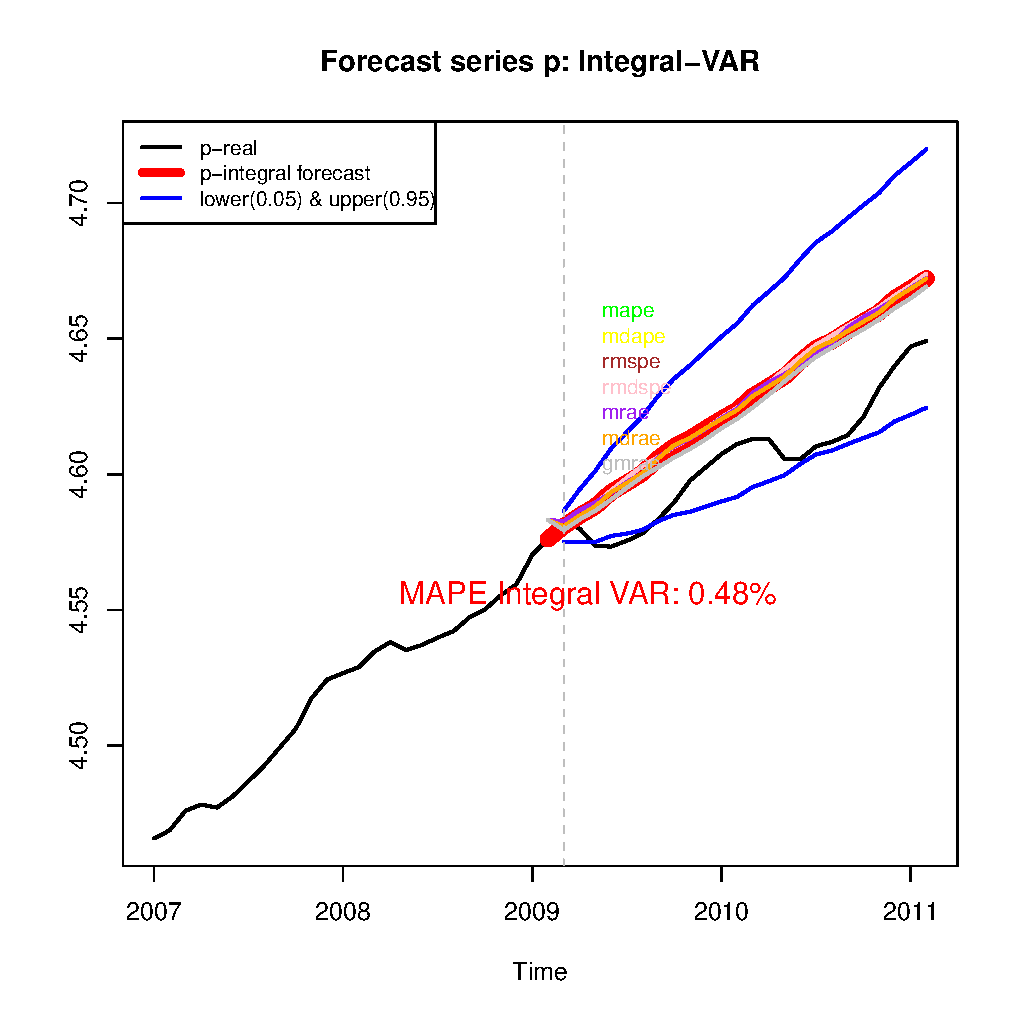
\includegraphics[scale=0.4]
      {figs/graph_3_v2.pdf}}
  \end{figure}
\end{frame}

\begin{frame}{$VAR-PLS$}
  \begin{figure}[htbp]
    \center{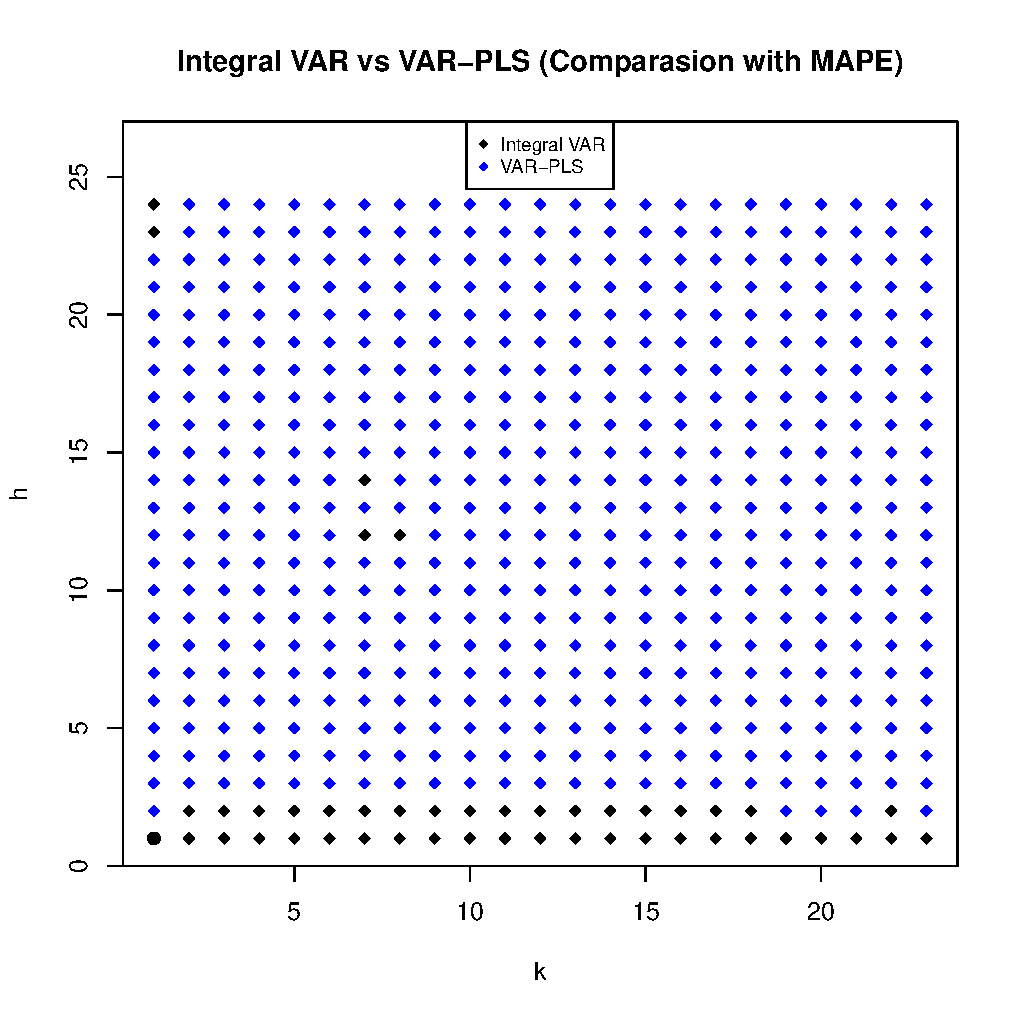
\includegraphics[scale=0.4]
      {figs/graph_4_v2.pdf}}
  \end{figure}
\end{frame}

\begin{frame}{$VAR-PLS$}
  En promedio, en 91.67\% de las veces, la representaci\'on PLS del VAR
  ... CHECAR AQU'I ESTA PARTE, CREO QUE LE FALTA UNA PALABRA EN EL
  BORRADOR VAR PLS V5.PDF.

  \bigskip

  El VAR-PLS parece ser un competidor atractivo con el VAR integral,
  que est\'a construido con fines de predicci\'on, teniendo la ventaja
  de proporcionar intervalos de confianza que incluyen la
  incertidumbre debida a la estimaci\'on de los par\'ametros. 
\end{frame}

\begin{frame}{}
  \begin{block}{}
    \begin{center}
      \vspace{3mm}
      {\Large Conclusiones}
      \vspace{3mm}
    \end{center}
  \end{block}
\end{frame}

\begin{frame}{Conclusiones}
  \begin{itemize}
  \item Presentamos un algoritmo alternativo de predicci\'on para un
    entorno multivariado, que toma en cuenta las dependencias entre
    las series $y_{t+j}$ con $y_t$, mediante un modelo PLS escrito
    como un modelo lineal con $X$ teniendo la representaci\'on $VARX$.
  \item Los resultados emp\'iricos para la inflaci\'on de M\'exico son
    bastante apropiados desde un punto de vista econ\'omico.
    \begin{itemize}
    \item VAR-PLS se contruy\'o con $p$ dado por el ajuste de un VARX,
      estimando en este caso, todos los $pK$ componentes posibles.
    \item Se construy\'o el intervalo de predicci\'on usando un
      m\'etodo Bootstrap.
    \end{itemize}
  \item El modelo VAR-PLS es una t\'ecnica multivariada atractiva para
    pronosticar este tipo de datos.
  \end{itemize}
\end{frame}

\begin{frame}{Conclusiones}
  Trabajo futuro:
  \begin{itemize}
  \item Buscar las relaciones impl\'icitas entre la cointegraci\'on
    (CCA) y PLS.
  \item Construir un VAR-PLS sin ajustar el modelo VAR, y comparar el
    pron\'ostico obtenido con el modelo VAR integral.
  \end{itemize}

\end{frame}

\begin{frame}{}
  \begin{block}{}
    \begin{center}
      \vspace{3mm}
      {\Large Gracias por su atenci\'on !}
      \vspace{3mm}
    \end{center}
  \end{block}
\end{frame}





\end{document}